\documentclass[]{article}
\usepackage{graphicx}
\usepackage{amsfonts,amssymb}
\usepackage[fleqn]{amsmath}
\usepackage[many]{tcolorbox}
\usepackage[%
margin=2cm,
includefoot,
bottom=2.55cm,
top=2.025cm,
headsep=0.5cm,
footskip=0.65cm
]{geometry}

\definecolor{myblue}{RGB}{0,46,142}

\newtcolorbox[auto counter]{mytheorem}[1][]{%
	enhanced jigsaw,
	colback=white,
	colframe=myblue,
	coltitle=myblue,
	fonttitle=\bfseries,
	sharp corners,
	detach title,
	enlarge left by=18mm,
	width=\linewidth-18mm,
	underlay unbroken and first={%
		\node[above,text=myblue,font=\bfseries,align=center] at ([xshift=-.5\textwidth,yshift=-7mm]interior.north) {\thetcbcounter};
	},
	breakable,
	pad at break=1mm,
	#1,
	code={\ifdefempty{\tcbtitletext}{}{\tcbset{before upper={\tcbtitle\par\medskip}}}},
}
\graphicspath{ {./images/} }


%opening
\title{L-15: Projections Onto Subspaces}
\author{Aahan Singh Charak\\Computer Science Grad}

\begin{document}
	
	\maketitle
	
	\section{2d Projections}
	\begin{center}
		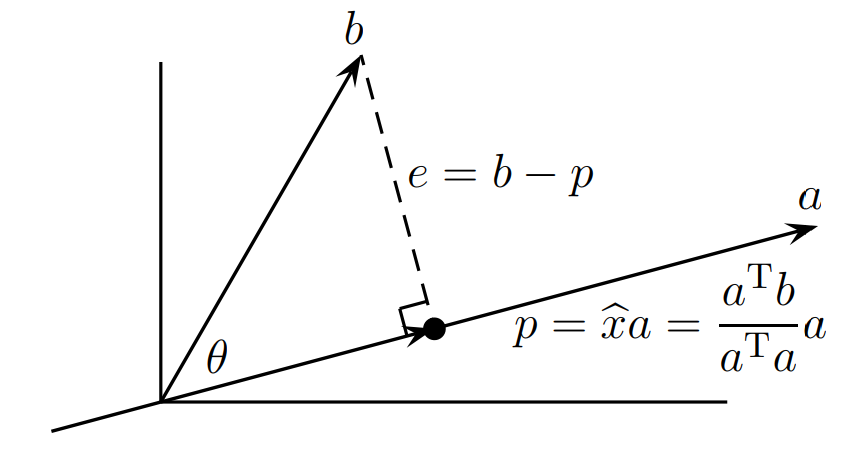
\includegraphics[scale=.25]{projection}
	\end{center}
	\vspace{10pt}
	
p = projection of b onto a\\

p=$\hat{x}a$\\

Also, a $\perp b \implies a \perp (b-\hat{x}a)$\\

$a_T(b-\hat{x}a)=0$\\

$\therefore \hat{x}a^Ta = a^Tb$\\
\begin{equation}
\hat{x}=\frac{a^tb}{a^ta}
\end{equation}

$\therefore p=a(\frac{a^Tb}{a^Ta})$\\

\begin{mytheorem}[title=Important Notes]
	\textbf{If b is doubled}, projection is doubled too.\\
	
	\textbf{If a is doubled}, nothing changes.(line onto which we are projecting remains the same.)
\end{mytheorem}

\vspace{10pt}

\subsection{Projection Matrix}

It is a matrix which acts on input b and projects it on a.\\

proj p=Pb\\
\begin{equation}
	\therefore P=\frac{aa^T}{a^Ta}
\end{equation}\\

\begin{mytheorem}[title = Properties of projection matrix]
	\begin{itemize}
		\item C(P) is the line through a. According to projection formula, we multiply P with b. So, we are always getting a projection on a.
		\item r(P)=1 (col*row=rank 1 matrix, a and it's transpose)
		\item $P=P^T$
		\item $P^2=P$ (self projection, obvious)
	\end{itemize}
\end{mytheorem}

\vspace{10pt}

\section{Why Project?}

Suppose, Ax=b has no solution. This means that b doesn't lie in A's column space. So, now we project b onto C(A) using a projection matrix.\\

Therefore, $A\hat{x}=p$, has a solution because we projected b onto C(A). p is the best solution, as it it closest to b, due to being a perpendicular projection.
\vspace{10pt}

\section{3d Projections}
	\begin{center}
	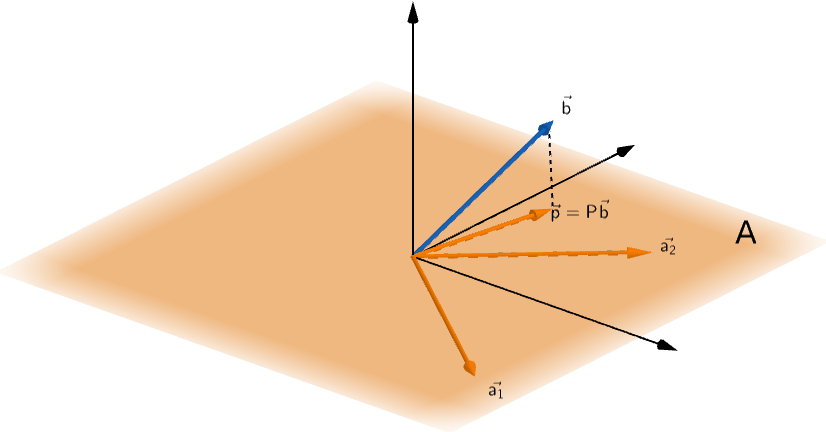
\includegraphics[scale=.4]{projection2}
\end{center}

\vspace{10pt}

a1 and a2 are the two basis vectors for the plane. They are independent and their linear combinations span the entire 2d plane.\\

Plane is the column space of A.\\

A=[a1 a2]\\

Now, $e \perp C(A)$\\

p can be written as a linear combination of a1 and a2.\\

$\therefore p =a1\hat{x1} + a2\hat{x2}$\\

$\therefore p=A\hat{x}$\\

Problem is to find the right combinations of the columns of A so that error vector is perpendicular to the plane.We have to find $\hat{x}$\\

Now, $e \perp plane \implies \ e \perp a1 \ and \ e \perp a2$\\

$a1^T(b-A\hat{x})=0 \ and \ a2^T(b-A\hat{x})=0$\\

Writing this in matrix form, we get :\\

\[
\begin{bmatrix}
a1^T \\
a2^T
	
\end{bmatrix}(b-A\hat{x})=0
\]\\

\begin{center}
	Or 
\end{center}

$A^T(b-A\hat{x})=0$\\

Now,\\

$A^TA\hat{x}=A^Tb$\\

$\therefore \hat{x}={(A^TA)}^{-1}A^Tb$\\

\begin{equation}
	p=A{(A^TA)}^{-1}A^Tb
\end{equation}
\vspace{10pt}

\subsection{3d Projection Matrix}
\vspace{10pt}

\begin{equation}
	P=A{(A^TA)}^{-1}A^T
\end{equation}
\vspace{10pt}
\begin{mytheorem}[title=Properties of 3d projection matrix]
	\begin{itemize}
		\item $P^T=P$
		\item $P^2=P$
	\end{itemize}
	
\end{mytheorem}

\vspace{10pt}
\section{Proofs}
\vspace{10pt}

\subsection{e is perpendicular to C(A)}
\vspace{10pt}
$A^Te=0$\\

$\therefore e \in N(A^T)$\\

$Now, N(A^T) \perp C(A)$\\

Therefore, e is perpendicular to C(A).\\

\textbf{Q.E.D}

\vspace{10pt}

\subsection{$P^2=P$}
\vspace{10pt}

$P^2=A{(A^TA)}^{-1}A^TA{(A^TA)}^{-1}A^T$\\

$=A{(A^TA)}^{-1}IA^T$\\

$=A{(A^TA)}^{-1}A^T=P$\\

\textbf{Q.E.D}


\end{document}